\section{Use Case Models}

\subsection{Scenarios}
We have chosen to select six specific scenarios to specify detailed. These are the scenarios that we think are the most important ones to get a good understanding of the more complicated features of the system. A list of the scenarios not further specified can be seen in appendix %\ref{sec:unspecified_use_case_models}.

The scenarios that we have chosen to focus on are shown below. We have chosen these since, we think that they represent some of the paramount parts of the system functionality, thus analysing these further will ensure that the main logic of the system is handled correctly.

\subsubsection{Scenario: Sell a Used Car to a Customer}
\HRule \\[0.4cm]
\textbf{Actors:} \texttt{Bob:Employee, Alice:Customer}\\
\HRule \\[0.4cm]
\textbf{Flow:} \\
\begin{enumerate}
\item Alice has chosen to get contacted by an employee of the used car lot about a nice Mercedes Benz she has seen on the website.
\item Bob, the employee, sees on the \texttt{DriveIT Windows Client} that Alice wants to get contacted about a given car.
\item Bob uses the \texttt{DriveIT Windows Client} to get contact information about Alice and to get some information about the car and gives Alice a call.
\item Bob and Alice talk on the phone and Bob succeeds in convincing Alice to buy the car.
\item Bob uses the system to make a sale with the car and Alice as the customer. He then sends a bill via email to Alice.
\end{enumerate}
\HRule \\[0.4cm]


\subsubsection{Scenario: Customer does not pick up. Employee sends e-mail}
\HRule \\[0.4cm]
\textbf{Actors:} \texttt{Robert:Employee, Joe:Customer}\\
\HRule \\[0.4cm]
\textbf{Flow:} \\
\begin{enumerate}
\item Robert sees that Joe wants to be contacted about a BMW.
\item Robert finds the info Joe has registered about himself in order to find his phone number.
\item Robert calls Joe, but Joe does not answer his telephone.
\item Robert looks in Joe's provided contact information again to find his e-mail address.
\item Robert sends an e-mail to Joe using an external e-mailing system.
\end{enumerate}
\HRule \\[0.4cm]


\subsubsection{Scenario: Customer wishes to find a car}
\HRule \\[0.4cm]
\textbf{Actors:} \texttt{Jane:Customer}\\
\HRule \\[0.4cm]
\textbf{Flow:} \\
\begin{enumerate}
 \item Jane, recently divorced, just had her tricycle stolen. With her regular commute of 36 miles each way, she spontaneously decides to buy a car.
 \item Jane faintly recalls the midnight infomercial she viewed the previous night while enjoying a gallon of Ben \& Jerrys and binge-watching Bridget Jones.
 \item After removing the heap of dirty clothes from her chair and finding her laptop, she swiftly types in the URL for DriveIT's used car lot web page.
 \item Upon entering the website, she is prompted with a landing page, where she can see some of the most recently added cars. She can also go to a more advanced view where she can sort cars by a list of criteria.
 \item She quickly sports the `sort by fuel type' criteria, and proceeds to locate the nearest blunt object to break her piggy bank.
 \item After counting her pennies, nickels and dimes she sets the `sort by fuel type'-field to diesel.
 \item Jane continues to click the `search' button and receives the list of 3 cars.
 \item Jane scrolls through the cars, looking at the specifications with her needs in mind, and ends up falling in love with the 1899 Horsey Horseless.
\end{enumerate}
\HRule \\[0.4cm]


\subsubsection{Scenario: Get Contacted by Employee}
\HRule \\[0.4cm]
\textbf{Actors:} \texttt{Alice:Customer, Bob:Employee}\\
\HRule \\[0.4cm]
\textbf{Flow:} \\
\begin{enumerate}
    \item Alice has been browsing the site of the used car dealership for a while and has found a car that she really likes.
    \item Since Alice is not in a hurry to get contacted, she decides that the wishes to be contacted by an employee of the dealership. 
    \item Alice presses the button named "Request to Get Contacted".
    \item Alice sees that the site where she requested to be contacted now says that a contact request has been sent.
\end{enumerate}
\HRule \\[0.4cm]


\subsubsection{Scenario: Put a New Used Car Up For Sale}
\HRule \\[0.4cm]
\textbf{Actors:} \texttt{Bob:Employee}\\
\HRule \\[0.4cm]
\textbf{Flow:} \\
\begin{enumerate}
\item The car lot has just purchased a new used car.
\item Bob needs to put the newly purchased car up for sale, so that the customers of the car lot can see and hopefully buy it.
\item Bob knows the make and model of the car, but not any other information. He uses the system to find additional information about the car. 
\item Bob has also taken a photo of the car, and uploads this to the page of the car. 
\item Bob has put all the information and photos he knows into the system, and saves the information. 
\item Bob double-checks that the car is saved and put up for sale. He is happy to see that that is the case.
\end{enumerate}
\HRule \\[0.4cm]


\subsubsection{Scenario: Customer Comments on a Car}
\label{sec:scenario-createcomment}
\HRule \\[0.4cm]
\textbf{Actors:} \texttt{John:Customer}\\
\HRule \\[0.4cm]
\textbf{Flow:} \\
\begin{enumerate}
\item John is browsing for cars, and while browsing he finds a Toyoto identical to one he once had himself.
\item Since John was very fond of the car he wants to leave a comment, letting other people know that it is a good car.
\item John is already signed in, and is therefore able to comment right away.
\item He writes fills in the title and description fields of the site. He then creates the comment.
\item John is now able to see his comment, and can delete or edit it if he so desires.
\end{enumerate}
\HRule \\[0.4cm]


\subsection{Use Case Model}
The use case model shows which actors can use which use-cases.\\

The unregistered customer can browse cars, see a detailed view of a specific car and browse employees.\\
A registered customer can do the same as the unregistered customer, but has access to modifying his or her user profile, as well as requesting to get contacted by an employee and the ability to comment on cars that are up for sale.
They also have the ability to see current contact requests that they have made and see all their previous orders made.\\

An employee can browse cars, view cars, browse employees, modify, create and delete user accounts, view the list of customers who wants to be contacted regarding cars for sale, sell cars, and create, modify and remove existing cars for sale on the web page.\\

The administrator is a special kind of employee who can access everything an employee can, as well as creating, modifying and removing other employees.\\

\begin{figure}[h!]
    \centering
        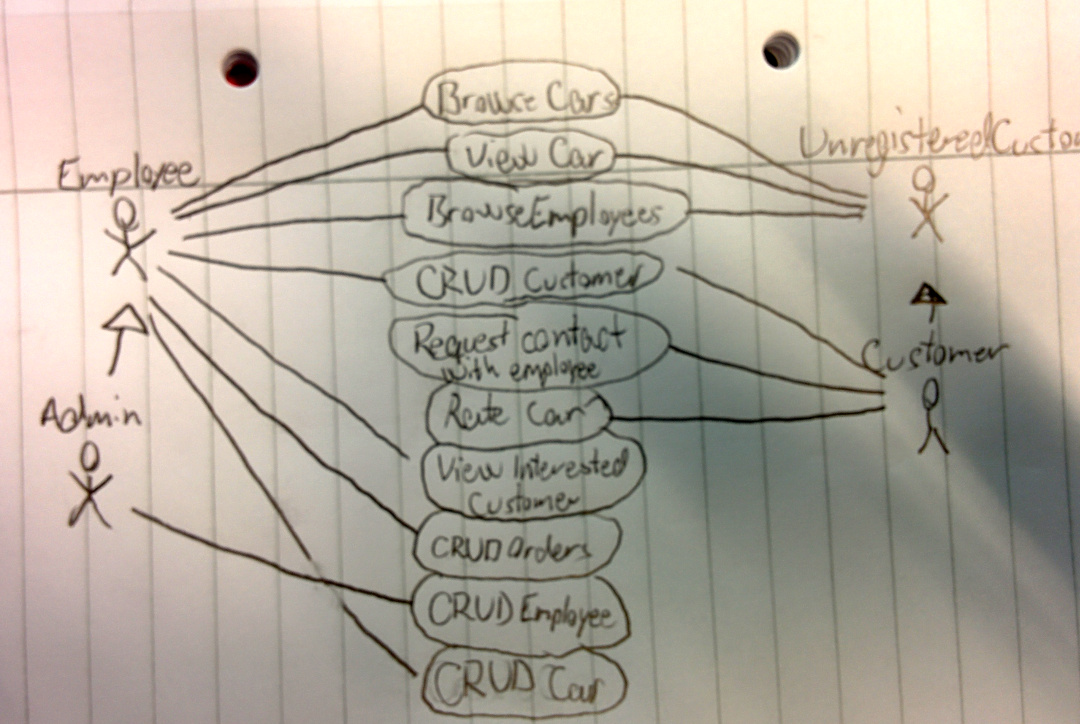
\includegraphics[scale=0.4]{Figures/UseCase-Model}\\
    \caption{The use case model - \texttt{Customer} inherits the unregistered customers cases, and the \texttt{Administrator} inherits from \texttt{Employee}}
  \label{fig:UseCaseModel}
\end{figure}

\section{Use Cases}

\subsubsection{UC-1 : Sell a Used Car to a Customer}
\label{create-order-use-case}
\HRule \\[0.4cm]
% Description
\textbf{Description:} The \texttt{Employee} creates an order when a \texttt{Customer} has decided to buy a specific car. \\
\HRule \\[0.4cm]
% Actors
\textbf{Actors:} \texttt{Employee, Customer}\\
\HRule \\[0.4cm]
% Preconditions
\textbf{Preconditions:} 
\begin{itemize}
    \item The \texttt{Customer} and the \texttt{Employee} has agreed upon a deal regarding the purchase of a specific car.
    \item The \texttt{Employee} has the \texttt{DriveIT Windows Client} available with an Internet connection.
\end{itemize}
\HRule \\[0.4cm]
% Postconditions
\textbf{Postconditions:}
\begin{itemize}
    \item A \texttt{Sale} has been successfully created and is persisted in the database.
    \item The \texttt{DriveIT Web Client} now shows that the car is sold, but leaves it available to view in the system for another week.
\end{itemize}
\HRule \\[0.4cm]
% Main success scenarios
\textbf{Main success scenario:}
\begin{enumerate}
    \item The \texttt{Employee} opens the 'Sales' view.
   
    \item The \texttt{Employee} presses the 'Create' button and selects the \texttt{Car}, \texttt{Customer}, and fills in the \texttt{Price} agreed upon.
    \item When all the requires fields to make a valid \texttt{Sale} is filled, the \texttt{Employee} clicks the 'Create Sale' button.
\end{enumerate}
\HRule \\[0.4cm]
\textbf{Exception Cases:}
\begin{itemize}
	\item If the \texttt{Customer} does not already exist in the system, then the \texttt{Employee} performs the use case \texttt{"Create Customer"}.
\end{itemize}
\HRule \\[0.4cm]
% Frequency
\textbf{Frequency:}
Daily \\
\HRule \\[0.4cm]




\subsubsection{UC-2 : Create User Account}
\label{create_account_use_cassse}
\HRule \\[0.4cm]
% Description
\textbf{Description:} The \texttt{Customer} registers on the \texttt{Web Client} \\
\HRule \\[0.4cm]
% Actors
\textbf{Actors:} \texttt{Customer}\\
\HRule \\[0.4cm]
% Preconditions
\textbf{Preconditions:} 
\begin{itemize}
    \item  The \texttt{Web Client} is initialized and the device initialising it is connected to the Internet.
    \item  The \texttt{Customer} is on the landing page of the \texttt{Web Client}.
\end{itemize}
\HRule \\[0.4cm]
% Postconditions
\textbf{Postcondition:}
\begin{itemize}
    \item The \texttt{Customer} has registered an account in the system.
    \item The \texttt{Customer} is able to login to the system.
\end{itemize}
\HRule \\[0.4cm]
% Main success scenarios
\textbf{Main success scenario:}
\begin{enumerate}
    \item  The \texttt{Customer} registers an account for the \texttt{Web Client}.
    \item  The \texttt{Customer} selects ´Register' in the main view of the \texttt{Web Client}.
    \item  The \texttt{Customer} inputs an e-mail address, first name, last name, and a password. He/she then selects the save button to save the account.
    \item  If the input is valid, the account is persisted and the \texttt{Customer} is logged in.
\end{enumerate}
\HRule \\[0.4cm]
% Frequency
\textbf{Frequency:}
Often \\
\HRule \\[0.4cm]



\usecase{
    title = {CreateCar},
    label = uc:createcar,
    description = {The \emph{Employee} Creates a car in the \texttt{DriveIT System} thereby making it available for sale.},
%    scope = {},
%    level = {},
    actors = {Initiated by\emph{Employee}},
%    stakeholders and interests = {},
    preconditions = {
        \item 1 The \emph{Employee} has some information about the new car.
    },
    postconditions = {
        \item 1 The car is in the \texttt{DriveIT System} and is available for sale on the \texttt{DriveIT Webclient}. 
    },
    main success scenario = {
        \item 1 The \emph{Employee} logs into the \texttt{DriveIT System}.
        \item 2 The \emph{Employee} finds the create car view.
        \item 3 The \emph{Employee} Fills data about the car in the view. 
        \item 4 The \emph{Employee} Checks the data and accepts it. The car is now succesfully in the system.
    },
    extensions = {
       \item 1 During item 3 in the main succes scenario, the \emph{Employee} should be able to fill in additional data about the car, by the help of an external system(CarQuery), using the model name.
    },
%    special requirements = {
%	    \item 1
%        \item 2
%		\\
%	},
    frequency of occurrence = Often,
    open issues = {It is unclear if the car should be immediately up for sale or if the \emph{Employee} should be able to choose what "state" the car should be in.}
}
\subsubsection{UC-3 : Create Car}
\label{create_car_use_case}
\HRule \\[0.4cm]
% Description
\textbf{Description:} An \texttt{Employee} uses the \texttt{Windows Client} to create a new car and thereby making it available for sale. \\
\HRule \\[0.4cm]
% Actors
\textbf{Actors:} \texttt{Employee}\\
\HRule \\[0.4cm]
% Preconditions
\textbf{Preconditions:} 
\begin{itemize}
    \item The \texttt{Employee} at least has the manufacturer and model of the car plus at least one picture.
    \item The \texttt{Employee} is signed in to the \texttt{Windos Client} and is connected to the Internet.
\end{itemize}
\HRule \\[0.4cm]
% Postconditions
\textbf{Postcondition:}
\begin{itemize}
    \item The \texttt{Car} is persisted in the database.
    \item The \texttt{Car} is available for sale on the \texttt{Web Client}.
\end{itemize}
\HRule \\[0.4cm]
% Main success scenarios
\textbf{Main success scenario:}
\begin{enumerate}
    \item The \texttt{Employee} signs in to the system.
    \item The \texttt{Employee} chooses the `Car' view and chooses the `Create' button.
    \item The \texttt{Employee} fills out the available data about the car. Given manufactorer and model, the \texttt{Employee} can choose to use the \texttt{Car Query API} to retrieve data about the given car.
    \item The \texttt{Employee} checks that the data is correct and submits the car.
\end{enumerate}
\HRule \\[0.4cm]
% Frequency
\textbf{Frequency:}
A couple of times a week \\
\HRule \\[0.4cm]



\usecase{
    title = {BrowseCars},
    label = uc:browsecars,
    description = {The (Unregistered)Customer wants to browse between cars},
%    scope = {},
%    level = {},
    actors = {Initiated by \emph{Customer} OR \emph{UnregisteredCustomer}},
%    stakeholders and interests = {},
    precondition = {The web-client (and the Web API) is online and available.},
%    preconditions = {
%        \item 1
%        \item 2
%        \item 3  
%    },
    postcondition = {The (Unregistered)Customer has found the cars he was looking for.},
%    postconditions = {
%        \item 1
%        \item 2
%        \item 3
%    },
    main success scenario = {
        \item The (Unregistered)Customer has opened the web-page.
    },
%    extensions = {
%        \item 1
%        \item 2
%        \item 3
%    },
%    special requirements = {
%	    \item 1
%        \item 2
%		\\
%	},
    frequency of occurrence = Often,
}

\subsubsection{UC-4 : Contact Interested Customer}
\label{contact-interested-customer-use-case}
\HRule \\[0.4cm]
% Description
\textbf{Description:} An \texttt{Employee} contacts a \texttt{Customer} who has requested to get contacted. \\
\HRule \\[0.4cm]
% Actors
\textbf{Actors:} \texttt{Employee, Customer}\\
\HRule \\[0.4cm]
% Preconditions
\textbf{Preconditions:} 
\begin{itemize}
    \item The \texttt{Windows Client} is online and the \texttt{Employee} is signed in to the system.
    \item There exists at least one \texttt{Contact Request} in the system.
\end{itemize}
\HRule \\[0.4cm]
% Postconditions
\textbf{Postcondition:}
\begin{itemize}
    \item The \texttt{Customer} who requested to get contacted has been contacted by the \texttt{Employee}.
\end{itemize}
\HRule \\[0.4cm]
% Main success scenarios
\textbf{Main success scenario:}
\begin{enumerate}
    \item The \texttt{Employee} navigates to the view of \texttt{Contact Requests}.
    \item The \texttt{Employee} chooses the oldest non contacted \texttt{Contact Request}, and open a detailed view of the request.
    \item The \texttt{Employee} contact the \texttt{Customer} through one of the means listed in the detailed view.
    \item Depending on the outcome of the communication between the two, the \texttt{Employee} either deletes the \texttt{Contact Request} or converts it into a \texttt{Sale}.
\end{enumerate}
\HRule \\[0.4cm]
% Frequency
\textbf{Frequency:}
Daily \\
\HRule \\[0.4cm]



\usecase{
    title = {RequestEmployeeContact},
    label = uc:req-emp-contact,
    description = {The \emph{User} wishes to be contacted by an \emph{Employee} about a car.},
%    scope = {},
%    level = {},
    actors = {Initiated by \emph{Customer}},
%    stakeholders and interests = {},
%    precondition = {},
    preconditions = {
    \item The \texttt{DriveIT System} is initialized and online.
    \item The \texttt{Customer} has found a car in the \texttt{DriveIT System} he/she wishes to be contacted about.
    },
%    postcondition = {},    
    postconditions = {
    \item The \emph{Customer} has submitted a request form.,
    \item The request-employee-contact-form has been registered in the \texttt{DriveIT System}.
    },
    main success scenario = {
       \item The \emph{Customer} has found a car he/she wishes to be contacted about.
       \item The \emph{Customer} fills out a request-employee-contact-form and submits it.
       \item The request-employee-contact-form is  registered in the \texttt{DriveIT System}.
       \item Any \emph{Employee} registered in the \texttt{DriveIT System} is now able to view and process the submission.
    },
%    extensions = {
%        \item 1
%        \item 2
%        \item 3
%    },
%    special requirements = {
%	    \item 1
%        \item 2
%		\\
%	},
    frequency of occurrence = Often,
    open issues = {It is unclear what is unclear},
}
